%! suppress = TooLargeSection
\documentclass[conf]{new-aiaa}
%\documentclass[journal]{new-aiaa} for journal papers

% \usepackage{lgrind}
% \usepackage{cmap}
% \usepackage[T1]{fontenc}

\usepackage{microtype}
\usepackage{amsmath}
\let\Bbbk\relax
\usepackage{amssymb}
\usepackage{gensymb}
\usepackage{graphicx}
\usepackage{pgf}
\usepackage{float}
% \usepackage{optidef}
\usepackage{ifdraft}
\usepackage[hyphens]{url}
\usepackage{hyperref}
\usepackage{enumitem}

\renewcommand{\labelitemii}{$\circ$}

\usepackage{eqexpl}
\eqexplSetIntro{where:} % set parenthesis in the left of the first item
\eqexplSetDelim{=} % set delimiter to "="

\usepackage{ar}

\usepackage{multicol}

\usepackage{siunitx}
\sisetup{}

\usepackage{longtable}
\usepackage{tabularx}
\usepackage{booktabs}
\usepackage{multirow}
\usepackage{tablefootnote}
\usepackage{tabularray}
\UseTblrLibrary{booktabs}
\UseTblrLibrary{counter}

% \usepackage{mdframed}
% \newmdenv[
%     topline=false,
%     bottomline=false,
%     skipabove=\topsep,
%     skipbelow=\topsep,
%     innerleftmargin=30pt,
%     innerrightmargin=30pt,
%     backgroundcolor=black!5
% ]{example}

% \usepackage{fontspec}
% \usepackage{mathspec}
%\setmathsfont(Digits,Latin,Greek)[Numbers={Proportional}]{EB Garamond}
% \setmathrm{EB Garamond}

\widowpenalty=300
\clubpenalty=300
\interfootnotelinepenalty=10000
\tolerance=9999
\emergencystretch=10pt
\hyphenpenalty=1000
\exhyphenpenalty=100

% \defaultfontfeatures{Mapping=tex-text}
% \newfontfamily{\smallcaps}[RawFeature={+c2sc,+scmp}]{EB Garamond}
% \setromanfont[Numbers={Proportional}, Ligatures={Common}]{EB Garamond}
% \setsansfont[Scale=MatchLowercase, BoldFont={Lato Bold}]{Lato Regular}
% \setmonofont[Scale=MatchLowercase]{Source Code Pro}



\usepackage{tikz}
\usetikzlibrary{positioning}
\usetikzlibrary{shapes.geometric}
\usetikzlibrary{shapes.arrows}
\usetikzlibrary{decorations.pathmorphing, decorations.pathreplacing, calc}
\usetikzlibrary{arrows.meta, positioning}

\usepackage{tikz-cd}
\tikzcdset{
    math mode=false
}

% \usepackage{minted}
% \usemintedstyle{pastie}
% %\usemintedstyle{jupyter_python}
% %\usemintedstyle{rainbow_dash}
% %\usemintedstyle{colorful}
% \setminted{
%     frame=lines,
%     framesep=2mm,
% %    numbers=left,
%     fontsize=\footnotesize,
% %    fontsize=\scriptsize,
%     autogobble=true,
%     baselinestretch=1.15,
%     breaklines,
%     linenos,
%     highlightcolor=cyan!15,
% }
% \setmintedinline{
%     breaklines
% }

% \PassOptionsToPackage{table,xcdraw}{xcolor}
\usepackage{xcolor}

% \definecolor{c1}{HTML}{64ACBE}
% \definecolor{c2}{HTML}{EE442F}
% \definecolor{c3}{HTML}{601A4A}

\definecolor{myorange}{RGB}{255, 165, 0}
\definecolor{mydarkseagreen}{RGB}{143, 188, 143}
\definecolor{mydodgerblue}{RGB}{30, 144, 255}

\colorlet{b}{red!13!white}
\colorlet{m}{yellow!20!white}
\colorlet{g}{green!18!white}


% \renewcommand{\theFancyVerbLine}{\sffamily
%     \textcolor[rgb]{0.8,0.8,0.8}{\scriptsize\oldstylenums{\arabic{FancyVerbLine}}}
% }


\usepackage{titlesec}
%\newcommand{\sectionbreak}{\clearpage}

\usepackage{caption}
\captionsetup[table]{skip=6pt}

\usepackage[numbers,sort&compress]{natbib}

\usepackage{adjustbox}

\usepackage[titletoc,title]{appendix}

% \usepackage{geometry}
% \geometry{
%     letterpaper,
%     left=1.0in,
%     right=1.0in,
%     top=1.0in,
%     bottom=1.0in
% }

% \usepackage{setspace}
% \setstretch{2}

\usepackage[inkscapearea=page]{svg}

\usepackage{subcaption}

\usepackage{afterpage}
\usepackage[section]{placeins}

\usepackage{nth}

%\usepackage{titling}
% \usepackage[palatino,nogrey]{quotchap}
% \definecolor{chaptergrey}{HTML}{64ACBE}


\usepackage{xstring}

% \makeatletter
%     \patchcmd{\@makechapterhead}{\thechapter}{%
%      \IfSubStr{ABCDEFGHIJKLMNOPQRSTUVWXYZ}{\thechapter}{\appname\,\thechapter}{\chapname\,\thechapter}
%     }
% \makeatother

% \newcommand{\appname}{{\fontfamily{phv}\fontsize{22pt}{26pt}\selectfont\raisebox{1em}{\textcolor{gray}{Appendix}}}} % set the appendix name <<<<<<<<<<<
% \newcommand{\chapname}{{\fontfamily{phv}\fontsize{22pt}{26pt}\selectfont\raisebox{1em}{\textcolor{gray}{\chaptername}}}} % set the chapter name <<<<<<<<<<<

\usepackage{authblk}

\usepackage{todonotes}
\setuptodonotes{inline,backgroundcolor=yellow!20,prepend,caption={TODO}}

\newcommand{\Rey}{\rm Re}
\newcommand{\M}{\rm M}
\newcommand{\Cp}{C_p}
\newcommand{\Cpo}{C_{p_0}}
\newcommand{\Cpm}{C_{p_{\rm min}}}
\newcommand{\Cpom}{C_{p_{0,\rm min}}}
\newcommand{\Cpcr}{C_{p_{\rm crit}}}
\newcommand{\Mcr}{M_{\rm crit}}
\newcommand{\Mdd}{M_{\rm dd}}
\newcommand{\Mi}{M_\infty}
\newcommand{\Ncr}{N_{\rm crit}}

\title{NeuralFoil: An Airfoil Aerodynamics Analysis Tool Using Physics-Informed Machine Learning}

\author{Peter Sharpe\footnote{PhD Candidate, AIAA Student Member} and R. John Hansman\footnote{T. Wilson Professor in Aeronautics, AIAA Fellow}}
\affil{Massachusetts Institute of Technology, Cambridge, MA}

\begin{document}

    \maketitle

    \begin{abstract}

        This work introduces \emph{NeuralFoil}, an open-source tool for rapid aerodynamics analysis of airfoils, similar in purpose to XFoil. NeuralFoil yields viscous and compressible airfoil aerodynamics results across an 18-dimensional space of airfoil shapes, possibly including control deflections, across a full $360\degree$ range of angles of attack, across chord Reynolds numbers from $10^2$ to $10^9$, for Mach numbers from zero to low transonic conditions, and with varying turbulence parameters. NeuralFoil's aerodynamic results match those of XFoil closely: on airfoils outside of NeuralFoil's training data, the mean absolute error of NeuralFoil's drag coefficient is 2.0\%. NeuralFoil computes both bulk quantities (lift, drag, etc.) as well as detailed flowfield behavior (boundary layer parameters, etc.) Moreover, NeuralFoil offers runtime speeds up to 1,000x faster than XFoil (for large batch analyses) and is amenable to gradient-based design optimization methods (e.g., $C^\infty$-continuous solutions, bounded computational cost, compatibility with automatic differentiation tools).

        For improved accuracy, parameter efficiency, and data efficiency, NeuralFoil uses a physics-informed machine learning approach. For example, the model components that handle attached flows are trained on synthetic data from $\approx$7 million XFoil analyses.
        This ``physics information'' includes both symmetries that are structurally embedded into the model architecture as well as feature engineering on inputs and outputs by leveraging domain knowledge.

        This work also develops a new approach to surrogate model uncertainty quantification, where the model directly learns and computes a model of its own uncertainty throughout the input space. This can be used to drive robust optimization with constraints on model error.

        This work discusses the model architecture, training, and performance of NeuralFoil on a variety of test cases, including an airfoil design optimization case study for the MIT Daedalus human-powered aircraft. In this case, NeuralFoil optimization is able to produce airfoils remarkably similar in performance and shape to expert-designed airfoils within seconds; these computationally-optimized airfoils provide a useful starting point for further expert refinement. NeuralFoil is implemented as a lightweight Python package with minimal dependencies, allowing easy installation across a variety of platforms.

    \end{abstract}

    \section{Nomenclature}

    {\renewcommand\arraystretch{1.0}
    \noindent\begin{longtable*}{@{}l @{\quad=\quad} p{5in}@{}}
                 $\beta$ & Prandtl-Glauert compressibility correction factor, defined as $\sqrt{1 - \Mi^2}$ \\
                 BL & boundary layer \\
                 CFD & computational fluid dynamics \\
                 $C_D$ & drag coefficient \\
                 $C_L$ & lift coefficient \\
                 $C_M$ & moment coefficient \\
                 $\Cp$ & local pressure coefficient (in the real compressible flow) \\
                 $\Cpo$ & local pressure coefficient in the equivalent incompressible flow \\
                 $\Cpm$ & minimum local pressure coefficient (in the real compressible flow) \\
                 $\Cpom$ & minimum local pressure coefficient in the equivalent incompressible flow \\
                 $c$ & airfoil chord \\
                 $c_\mathcal{D}$ & dissipation coefficient \\
                 $c_f$ & skin friction coefficient \\
                 $c_{\rm lower}$ & Kulfan (CST) shape parameters associated with the airfoil's lower surface \\
                 $c_{\rm upper}$ & Kulfan (CST) shape parameters associated with the airfoil's upper surface \\
                 $\gamma$ & ratio of specific heats of the working fluid; 1.4 for air near standard conditions \\
                 $H$ & BL shape parameter, defined as $\delta^*/\theta$ \\
                 $H^*$ & BL kinetic energy shape parameter, defined as $\theta^*/\theta$ \\
                 LE & airfoil leading edge \\
                 $M$ & local Mach number \\
                 $\Mi$ & freestream Mach number \\
                 $\Mcr$ & critical Mach number, defined as the lowest freestream Mach number where any point in the flow is supersonic \\
                 $M_{\rm dd}$ & drag-divergent Mach number, defined as the freestream Mach number above which drag begins to rise rapidly \\
                 $\nu$ & kinematic viscosity \\
                 $\Ncr$ & BL critical amplification factor (affected by surface roughness, freestream turbulence) \\
                 RANS & Reynolds-averaged Navier-Stokes equations \\
                 $\Rey_c$ & chord Reynolds number, defined as $u_\infty c / \nu$ \\
                 $\Rey_\theta$ & momentum-thickness Reynolds number, a local BL quantity defined as $\theta u_e / \nu$ \\
                 $s$ & coordinate along the airfoil surface, starting at the TE and proceeding over the top surface \\
                 $\theta$ & BL momentum thickness \\
                 $\theta_{\rm TE}$ & Trailing-edge angle \\
                 TE & airfoil trailing edge \\
                 $u_e$ & BL edge velocity \\
                 $u_\infty$ & freestream velocity magnitude \\
                 $u_{\rm max}$ & maximum velocity magnitude at any point in the flow field \\
                 $x_{\rm tr}$ & actual laminar-turbulent transition location, relative to the leading edge; appropriate suffixes denote top- and bottom-surface measures \\
                 $x_{\rm tr, forced}$ & location of any forced trips for bypass transition (e.g., turbulators, rivets), if present; $x_{\rm tr, forced} / c = 1$ if absent\\
                 $x / c$ & nondimensional distance along the airfoil chord ($\text{LE} \rightarrow 0$, $\text{TE} \rightarrow 1$) \\
                 $y / c$ & nondimensional distance normal to the airfoil chord (LE and TE at 0, barring any control surface deflections) \\
                 $z_{\rm in}$ & input latent space vector \\
                 $z_{\rm out}$ & output latent space vector \\
    \end{longtable*}}


    \section{Introduction}

    In conceptual aircraft design, the problem of shaping a typical wing is usually decomposed into two parts: planform design and airfoil design. The latter, which is the focus of this work, is a multidisciplinary design problem that requires consideration of a variety of aerodynamic, structural, and manufacturing objectives and constraints. A non-exhaustive list of major considerations could include:
    \begin{itemize}
        \item Profile drag across the expected operating range of the airfoil (spanning lift coefficients, Reynolds numbers, and Mach numbers), including adequate off-design performance \cite{drela_pros_1998};
        \item Pitching moment and aft-camber coefficients, which can drive tail sizing (modifying trim drag), affect divergence speed;
        \item Hinge moments and control effectiveness of any control surfaces, which drive actuator design and weight;
        \item Stall behavior, which can affect handling qualities and safety;
        \item Thickness at various points, in order to accommodate fuel volume and required structural members to resist failure (e.g., by bending, buckling, divergence, flutter, or control reversal);\cite{sharpe_tailerons_2023}
        \item Sensitivity to boundary layer performance, freestream turbulence, and trips, all of which impose constraints on surface finish, cleanliness, and manufacturing tolerances \cite{eleshaky1993airfoil, selig_highlift_1997, liebeck1973class};
        \item Peak suction pressures, which affect the critical Mach number in transonic applications or cavitation in hydrodynamic applications;
        \item Shock stability and buffet considerations in transonic applications;
        \item Manufacturability, which might include flat-bottom airfoil sections, strictly-convex airfoil shapes (e.g., to accommodate shrink-coverings, which are common in ultra-lightweight applications \cite{drela_lowreynoldsnumber_1988}), or restrictions on trailing-edge angle.
    \end{itemize}

    These airfoil design drivers often differ considerably at different locations along the span of the wing, which often leads to a family of airfoils being used in the design of a given wing. To fulfill such design requirements, a designer will typically either find an existing airfoil or design a new airfoil. Given the specificity of the requirements illustrated in the list above, designing bespoke airfoils can yield considerable performance improvement.

    Currently, three approaches are commonly used to computationally design new airfoils: inverse design methods, direct manual methods, and optimization methods. In the inverse design approach, popularized by Drela's XFoil code \cite{drela_xfoil_1989} and Eppler's Profil code \cite{profil, tao_bs_thesis}, conformal mapping methods are used to reconstruct a new airfoil shape from a user-specified pressure distribution. This has the benefit of allowing the engineer to directly operate on the most relevant aerodynamic quantities, and it produces considerable design insight. However, it can be time-consuming to produce airfoils that satisfy non-aerodynamic constraints (e.g., manufacturability, spar thickness) due to the lack of direct control here. Conformal mapping methods are also only strictly applicable to potential-flow-governed regions, so the specified pressure distribution is often only the inviscid, rather than viscous (true) pressure distribution\footnote{This can be alleviated by using nonlinear optimization to target the viscous pressure distribution, albeit with reduced numerical robustness.}.

    In the direct manual method (or ``geometric design'' method, using parlance from XFoil), an engineer formulates an airfoil shape directly and modifies this iteratively by hand. Aerodynamic analysis is performed by any code that will perform the forward problem (geometry $\rightarrow$ aerodynamics), such as XFoil, MSES \cite{mses}, or any RANS-based CFD code \cite{adler_cfd_2022}. This allows for easier satisfaction of non-aerodynamic constraints. However, it is predictably more difficult to directly target aerodynamic quantities. Significant user expertise is also required to identify the most relevant geometric parameters and to make effective changes to the airfoil shape.

    In the optimization approach, a parameterized airfoil shape is optimized to minimize a cost function and satisfy specified constraints (which may be both aerodynamic and non-aerodynamic). At first glance, this appears to be an automation of the direct manual method. However, Drela and others note the surprising difficulty of posing the correct optimization problem \cite{drela_pros_1998, kroo_multidisciplinary_1997}, so this approach often requires just as much (if not more) human expertise than the direct manual method. As stated by Drela \cite{drela_pros_1998}, optimization-based airfoil design ``is still an iterative cut-and-try undertaking. But compared to [direct] techniques, the cutting-and-trying is not on the geometry, but rather on the precise formulation of the optimization problem.'' To support this, Drela gives compelling case studies of how airfoil design optimization can go awry in the absence of user review and care.\footnote{Some codes, like LINDOP \cite{mses}, alleviate this somewhat by using a hybrid of the direct and optimization approaches: update directions are computed by an optimizer, but the actual changes are reviewed and implemented by a human between iterations.}However, despite these cautionary notes, the optimization-based airfoil design approach also offers compelling benefits: resulting airfoil performance can equal that of airfoils by an expert \cite{drela_pros_1998}, particularly on problems with unique or otherwise non-intuitive constraints. This optimization process can also require orders of magnitude less engineering time, and it provides a systematic and disciplined approach that is especially suited to the most challenging design problems \cite{he2019robust}.

    In all of these methods, some form of a computational tool for airfoil aerodynamics analysis is required. For subsonic airfoils, the gold standard of such tools is XFoil \cite{drela_xfoil_1989}. Morgado et al. find that XFoil is more accurate than RANS-CFD-based tools in this regime \cite{morgado2016xfoil}, yet it has a computational cost that is roughly 1,000x lower -- a testament to the power of its modeling approach, which strongly-couples integral boundary layer and potential flow methods. A complete description of this modeling approach is available in Drela's \textit{Aerodynamics of Viscous Fluids} \cite{drela_aerodynamics_2019}, and in recent state-of-the-art work by Zhang \cite{zhang_threedimensional_2022, zhang_nonparametric_2017}. However, despite XFoil's many strengths, it has several attributes that make it less-than-ideal for directly driving numerical optimization studies \cite{adler_cfd_2022}. Among these:

    \begin{itemize}
        \item XFoil is not guaranteed to produce a solution. When an ``ambitious'' calculation is attempted, XFoil often fails to provide a converged solution; the unconverged result often has wildly-diverging values and is effectively unusable. In some cases, calculations can lead to infinite loops or process crashes due to unhandled exceptions. While this is acceptable in certain applications (e.g., manual direct analysis), it is generally unacceptable for use in numerical optimization. Instead, optimization strongly benefits from a robust analysis tool that always produces a result, even if that result has degraded accuracy; this allows the analysis to steer the optimizer back towards the design space of reasonable airfoils \cite{he2019robust}. A particularly useful attribute is when the model is deliberately made to be slightly pessimistic (e.g., overestimate drag) in regions of the design space with high uncertainty, adding further optimization pressure towards reasonable designs with low performance uncertainty.
        \begin{itemize}
            \item More generally, design optimization is not the only application that strongly benefits from an aerodynamics analysis tool that always produces an answer. Other examples where a non-answer, infinite loop, or crashed process are unacceptable include real-time control (e.g., as an aerodynamic model for a model-predictive controller onboard an aircraft) and flight simulation.
        \end{itemize}
        \item XFoil solutions are not necessarily unique, and slightly different solutions can be obtained for the same analysis problem (airfoil shape, angle of attack, and Reynolds and Mach numbers). In practice, this manifests as an effective hysteresis depending on whether angle of attack is swept up or down. This flow non-uniqueness is in fact a real physical\footnote{For example, flow over an airfoil may separate as its angle of attack increases past $12\degree$, but it may not fully reattach until the angle of attack descends back to below $11\degree$} effect \cite{jameson_airfoils_1991, kuzmin2012non, he2019robust}. However, this non-uniqueness can be exceptionally problematic for numerical optimization, as an infinitesimal change in an input parameter can result in the solution jumping to a different Newton basis of attraction. Therefore, there is no limit to how sensitive performance can be to input parameters (which hampers techniques like finite-differencing for gradient-based optimization).
        \item XFoil solutions are non-smooth\footnote{precisely, they are $C^0$ continuous but not $C^1$ continuous} with respect to input parameters, which makes it fundamentally incompatible with gradient-based optimization. (Any attempt to directly optimize XFoil results with gradient-based methods invariably results in premature stopping at a local minima.) Interestingly, this is a consequence of how laminar-turbulent transition is handled by XFoil's integral boundary layer solver. This solve requires the use of laminar and turbulent boundary layer \emph{closure models}, which are curve-fitted functions that yield various necessary quantities ($H^*$, $c_f$, $c_\mathcal{D}$, etc.) of the von Karman integral momentum and kinetic energy equations as a function of the two values that parameterize the boundary layer ($H$, $\Rey_\theta$). The laminar and turbulent versions of these functions differ. XFoil implements a cut-cell approach on the transitioning interval, which restores $C^0$-continuity (i.e., transition won't truly ``jump'' from one node to another discretely); however, a sharp change in gradient occurs whenever an individual node switches its equation from laminar to turbulent. Adler et al. provide a graphical depiction of this phenomenon \cite{adler_cfd_2022}.
        \item Most interfaces between an optimizer and XFoil communicate through a series of text files (i.e., hard disk), rather than by sharing data in memory (i.e., RAM). Given the quick speed of an individual XFoil run, this input-output overhead imposes a significant performance penalty. While this programming-language-agnostic interface is arguably one of the reasons for XFoil's long-enduring popularity, it comes at the cost of runtime performance if the tool is to be used in a high-throughput setting (e.g., for design optimization).
    \end{itemize}

    This motivates the development of a new airfoil aerodynamics analysis tool that captures the advantages of XFoil (accuracy, speed) while mitigating these drawbacks (i.e., incompatibility with gradient-based optimization). In recent years, many fields have benefited from a hybrid data-and-theory approach, where data-driven models are used to augment traditional physics-based models with learned closures. This work presents a similar physics-informed approach as applied to analyzing airfoil aerodynamics.

    % TODO write about other physics-informed ML approaches, webfoil?


    \section{NeuralFoil Tool Description and Methdology}

    \subsection{Overview}

    % Fundamentally, NeuralFoil consists of physics-informed neural networks trained on tens of millions of XFoil runs, with appropriate physics-based constraints structurally embedded into the model architecture. NeuralFoil focuses on estimating bulk quantities (e.g., lift and drag forces) rather than flow-field quantities (e.g., pressure distribution), as the former are most directly relevant to conceptual aircraft design.

    NeuralFoil is a tool for rapid aerodynamics analysis of airfoils, similar in purpose to the end-user as XFoil \cite{drela_xfoil_1989}. A precise list of inputs and outputs to NeuralFoil is given in Figure \ref{fig:neuralfoil_io}.

    \begin{figure}[H]
        \centering
        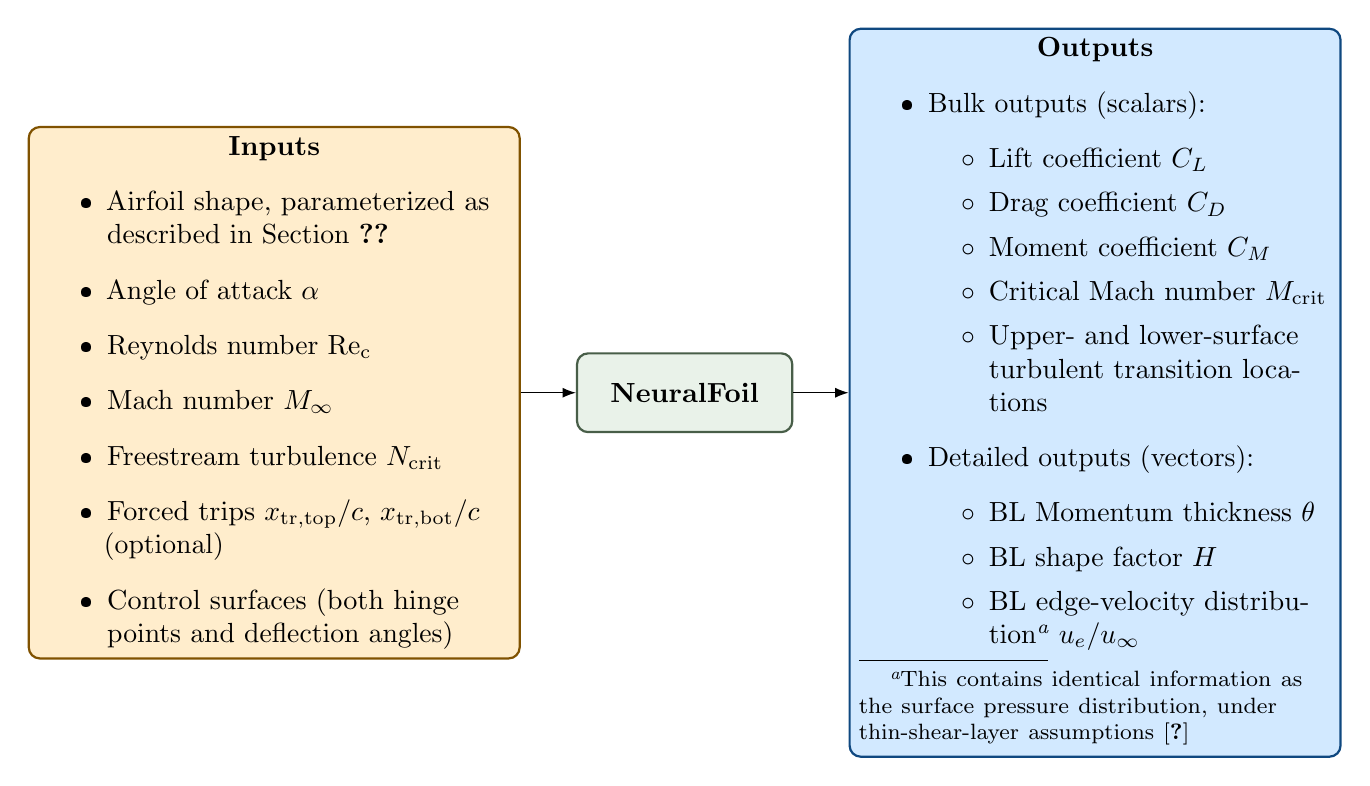
\begin{tikzpicture}[
            node distance=0.7 cm and 0.7 cm,
            auto,
            box/.style={
                rectangle,
                rounded corners,
                draw=#1!50!black,
                fill=#1!20,
                thick,
                text width=6cm,
                align=center,
                minimum height=1cm
            },
            title/.style={font=\bfseries},
            list/.style={align=left}
        ]

            % Nodes
            \node[box=myorange] (inputs) {
                \textbf{Inputs}
                \begin{itemize}
                    \item Airfoil shape, parameterized as described in Section \ref{sec:airfoil-parameterization}
                    \item Angle of attack $\alpha$
                    \item Reynolds number $\Rey_c$
                    \item Mach number $\Mi$
                    \item Freestream turbulence $\Ncr$
                    \item Forced trips $x_{\rm tr, top} / c$, $x_{\rm tr, bot} / c$ (optional)
                    \item Control surfaces (both hinge points and deflection angles)
                \end{itemize}
            };

            \node[box=mydarkseagreen, right=of inputs, text width=2.5cm] (neuralfoil) {
                \textbf{NeuralFoil}
            };

            \node[box=mydodgerblue, right=of neuralfoil] (outputs) {
                \textbf{Outputs}
                \begin{itemize}
                    \item Bulk outputs (scalars):
                    \begin{itemize}
                        \item Lift coefficient $C_L$
                        \item Drag coefficient $C_D$
                        \item Moment coefficient $C_M$
                        \item Critical Mach number $\Mcr$
                        \item Upper- and lower-surface turbulent transition locations
                    \end{itemize}
                    \item Detailed outputs (vectors):
                    \begin{itemize}
                        \item BL Momentum thickness $\theta$
                        \item BL shape factor $H$
                        \item BL edge-velocity distribution\footnote{This contains identical information as the surface pressure distribution, under thin-shear-layer assumptions \cite{drela_xfoil_1989}} $u_e/u_\infty$
                    \end{itemize}
                \end{itemize}
            };

            % Arrows
            \draw[-Latex] (inputs) -- (neuralfoil);
            \draw[-Latex] (neuralfoil) -- (outputs);
        \end{tikzpicture}
        \caption{User-facing inputs and outputs of the NeuralFoil model.}
        \label{fig:neuralfoil_io}
    \end{figure}

    \noindent Reasonable aerodynamics estimates can be expected:
    \begin{itemize}
        \item For any practical airfoil shape that can be analyzed with XFoil\footnote{only single-element airfoils are allowed}, including modifications for trailing-edge control surface deflections up to substantial deflections (e.g., $\pm 40\degree$)
        \item Across the $360\degree$ angle of attack range, by leveraging analytical post-stall models regressed from high-$\alpha$ wind tunnel data by Truong \cite{truong_analytical_2020}
        \item Across the range of Reynolds numbers associated with practical external aerodynamics flows ($10^2$ to $10^9$), with physically-sensible extrapolation even beyond this range (e.g., Stokes flow limit)
        \item At subsonic and low-transonic Mach numbers, ranging from zero to slightly above the drag-divergent Mach number
    \end{itemize}

    \noindent NeuralFoil has a mathematical form that is fully explicit (i.e., no iterative solvers are used; there is no value-dependent code execution). This guarantees that a deterministic result is returned in bounded computational time and without any need for initial guesses. As discussed in Section TODO, this also makes compatability with automatic differentiation frameworks much more straightforward, as the computational graph is static for any input. At a high level, the mathematical model within NeuralFoil consists of the following main steps:

    \begin{enumerate}
        \item \textbf{Pre-solve}: Converts the user-supplied airfoil shape into the required parameterization (including any control surfaces, which are made part of the airfoil geometry as described in Section \ref{sec:control-surfaces})
%        \item Temporary restriction to the incompressible flow case (i.e., input Mach is set aside for now; addressed later)
        \item \textbf{Encoding}: Transforms all inputs (except Mach number, which is treated later) into an appropriate input vector space for the neural network. This is performed using prescribed functions based on domain knowledge.
        \item \textbf{Learned Model}: A learned neural network maps from this latent vector space to another latent vector space.
        \item \textbf{Decoding}: Transforms the outputs of this neural network back into the space of user-facing outputs. This is also performed using prescribed functions based on domain knowledge.
        \item \textbf{Uncertainty quantification, model fusion, and extrapolation}: Based on the neural network's self-reported trustworthiness (via a process described in Section \ref{sec:uq}), the network's results are merged with analytical models for airfoil behavior in massively-separated flow conditions.
        \item \textbf{Compressibility correction}: The solution is corrected for non-zero Mach numbers using analytical methods, as described in Section \ref{sec:compressibility}.
    \end{enumerate}

    \noindent In the following sections, we will describe each of these steps in more detail.

    \subsection{Pre-Solve}
    \label{sec:airfoil-parameterization}

    \subsubsection{Airfoil Geometry Parameterization}

    NeuralFoil accepts user-specified airfoil shapes in a variety of common formats -- for example, as an array of $(x, y)$ coordinates, as a standard coordinate-array \texttt{*.dat} file, as a series of CST parameters, or as an Airfoil-class object within the AeroSandbox aircraft design optimization framework \cite{sharpe_aerosandbox_2021}.

    Underneath this interface layer, NeuralFoil converts this specified airfoil geometry to an 8-parameter-per-side CST (Kulfan) parameterization, including Kulfan's added leading-edge-modification (LEM) and trailing-edge thickness parameter \cite{kulfan_universal_2008, kulfan_modification_2020}. This gives a total of 18 parameters to describe a given airfoil shape, which are illustrated in Figure \ref{fig:neuralfoil_parameterization}. This parameterization family was chosen due to work by Masters \cite{masters_geometric_2017} and others, which shows that this is one of the most parameter-efficient representations of airfoil shape. Kulfan's parameterization is strongly related to an orthogonal polynomial decomposition using Bernstein polynomials. Because of this, the format is interpretable: it is a linear combination of mode shapes, each of which is roughly locally-supported\footnote{this contrasts with approaches such as taking an SVD over a standard airfoil database, which creates less-interpretable mode shapes}. Another benefit of the CST parameterization is interoperability, as it is commonly implemented in existing aerospace tools such as OpenVSP \cite{mcdonald_open_2022}.

    The CST parameterization allows for varying numbers of degrees of freedom. An 18-parameter representation was chosen based on the work of Masters \cite{masters_geometric_2017}, which shows that error in aerodynamic force prediction decreases substantially near this threshold. Thus, this parameterization strikes an acceptable balance between parameterization error and dimensionality. The 18-parameter representation also corresponds to one of the initially-proposed discretization levels proposed by Kulfan \cite{kulfan_universal_2008} (labeled in this work as ``BPO8''), so this parameterization is a natural choice for compatibility with existing airfoil design tools.

    Conversion of user-specified airfoils to this format for NeuralFoil to use is automatically and efficiently handled as a least-squares fitting problem.

    \begin{figure}[h]
        \centering
        \adjustbox{trim=0cm 1.5cm 0cm 0cm}{
            \includesvg[width=0.8\textwidth]{../../media/kulfan_parameterization_illustration.svg}
        }
        \caption{Geometry input parameterization used by NeuralFoil. Parameterization is an 18-parameter CST (Kulfan) parameterization \cite{kulfan_universal_2008, kulfan_modification_2020, masters_geometric_2017}. Each colored line in the figure represents a mode shape associated with one of these parameters; modes are linearly combined to form the airfoil shape.}
        \label{fig:neuralfoil_parameterization}
    \end{figure}

    \subsubsection{Control Surfaces}
    \label{sec:control-surfaces}

    Control surfaces are handled as a degenerate problem by re-normalizing the deflected airfoil shape. This is illustrated in Figure \ref{fig:control_surface_decomposition}. In step 1, an example airfoil is given. In step 2, a user-specified control surface deflection is applied. In step 3, the airfoil is re-normalized by applying the necessary similarity transformation (rotation, translation, and scaling) such that the leading-edge and trailing-edge locations are placed at their standard $(0, 0)$ and $(1, 0)$ locations in chord-normalized airfoil coordinates. The geometric rotation required for this re-normalization is later applied as a change in the effective angle of attack, $\Delta\alpha$. For consistency, the scaling factor required for this operation is also later used to scale the input Reynolds number appropriately, though the effect of this Reynolds scaling is typically minor. Finally, The resulting pitching moment must also be adjusted to account for shifting of the force center due to translation during re-normalization.

    \begin{figure}[h]
        \centering
        \includesvg[width=\textwidth]{../../studies/control_surface_decomposition.svg}
        \caption{Illustration of the automatic procedure for handling control surface deflections in NeuralFoil.}
        \label{fig:control_surface_decomposition}
    \end{figure}

    Also visible in Figure \ref{fig:control_surface_decomposition} is the geometric effect of restricting the airfoil shape to the space of CST-parameterized airfoils, which is performed along with the re-normalization step between steps 2 and 3. The effect of this is that the sharp corners associated with the control surface deflection are smoothed out, which is a consequence of the smooth mode shapes associated with the CST parameterization. The rationale behind accepting this loss of fidelity here is that the control surface deflection invariably causes a turbulent transition at the deflection point on the suction side, regardless of whether the sharp or smoothed geometry is used. Because the turbulent boundary layer that follows the hinge is less sensitive to the pressure distribution (and hence, airfoil shape), the loss of geometric accuracy is less significant. Nevertheless, some loss of aerodynamic accuracy is to be expected.

    To quantify this loss of accuracy, Figure \ref{fig:control_surface_accuracy} shows airfoil aerodynamics results obtained by both NeuralFoil and XFoil for various control surface deflections. Notably, reasonably close agreement is seen even for control surface deflections as aggressive as $\pm40 \degree$.

    \begin{figure}[H]
        \centering
        \includesvg[width=\textwidth]{../../studies/control_surface_accuracy.svg}        \caption{Accuracy of NeuralFoil on an airfoil with large control surface deflections. Here, we show aerodynamics results from both NeuralFoil and XFoil on a NACA0012 airfoil at $\Rey_c = 10^6$ and $\alpha = 0\degree$, with varying control surface deflections on a trailing-edge flap hinged at $x/c=0.70$.}
        \label{fig:control_surface_accuracy}
    \end{figure}

    \subsection{Encoding, Learned Model Architecture, and Decoding}

    After geometry parameterization, NeuralFoil transforms the user-facing inputs and outputs shown in Figure \ref{fig:neuralfoil_io} into intermediate vector spaces (latent spaces) that are more amenable to learning by a neural network. These latent spaces are carefully parameterized such that learned model has a close-to-affine mapping of inputs to outputs. Effectively, this is feature engineering using domain-specific knowledge.

    This encoding/decoding scheme has two major effects. First, it substantially increases model's parameter efficiency\footnote{i.e., test-set accuracy, relative to the number of parameters (which represent model complexity and computational cost)}, since the training data has fewer nonlinearities in this latent space. Secondly, the combination of encoding functions, model architecture, and decoding functions can be used to guarantee physically-sound extrapolation beyond the dataset \cite{xu_how_2021}. An example that illustrates both of these effects is the encoding of both the $\Rey_c$ input and the $C_D$ output into logspace. This means that an affine model in the latent space corresponds to a power-law $C_D(\Rey_c)$ model in user-facing space, which is a relationship supported by physical theory for both laminar and turbulent flows (e.g., Falkner-Skan and Schlichting boundary layer models \cite{drela_aerodynamics_2019}).

    \subsubsection{Encoding}

    The user-facing input space (shown in Figure \ref{fig:neuralfoil_io}) is transformed into the following input latent space, which is effectively what is seen by the neural network:

    \begin{equation}
        z_{\rm in} = \text{Affine}\left( \begin{bmatrix}
                                             \text{Airfoil shape (18 parameters)} \\
                                             \sin(2 \alpha)                       \\
                                             \sin^2(\alpha)                       \\
                                             \cos(\alpha)                         \\
                                             \ln(\Rey_c)                          \\
                                             \Ncr                                 \\
                                             x_{\rm tr, top, forced}              \\
                                             x_{\rm tr, bot, forced}              \\
        \end{bmatrix} \right)
        %label
        \label{eq:encoding}
    \end{equation}

    The resulting $z_{\rm in}$ is 25-dimensional. Note that the inputs described in Equation \ref{eq:encoding} also undergo a simple elementwise affine transformation. This transformation is such that the distribution of typical inputs in the latent space has a mean of roughly zero and a standard deviation of roughly one\footnote{This normalization is performed on the basis of the training data, described later in Section TODO}. Scaling and shift factors are available in the open-source codebase, for the interested reader. The purpose of this transformation is to improve the stability of the neural network training process, as well as to improve the performance of the weight-decay-based regularization strategy that is later used during training to improve generalization (described in Section \ref{sec:training-process}).

    In addition to the previously-discussed log-space transformation of Reynolds number, some nonlinear transformations on the angle of attack $\alpha$ are present and merit discussion as well. Encoding of angle of attack into a purely-trigonometric representation embeds the periodic nature of the problem into the model architecture. For example, model evaluation at $\alpha=0\degree$ and $\alpha=360\degree$ are structurally identical, as these are encoded to the same location in the input latent space. The $\sin(2\alpha)$ and $\sin^2\alpha$ terms are directly proportional to common post-stall analytical models of lift and drag, respectively (such as those by Hoerner and Truong \cite{hoerner_fluiddynamic_1992, truong_analytical_2020}). The goal of this representation is to improve generalization performance in massively-separated flow conditions, where training data is scarce.

    \subsubsection{Learned Model Architecture}
    \label{sec:learned-model-architecture}

    After encoding inputs into an input latent space, NeuralFoil processes these inputs through a feedforward neural network (i.e., multilayer perceptron). NeuralFoil offers eight different deep neural network models, which offer a tradeoff between accuracy and computational cost. This tradeoff is implemented as differences in the number and size of hidden layers, which are detailed in Table \ref{tab:model-sizes} for each model.

    \begin{table}[H]
        \centering
        \caption{Neural network model sizes offered in NeuralFoil, offering a trade between accuracy and speed.}
        \label{tab:model-sizes}
        \begin{tabular}{lll}
            \toprule
            Model        & Hidden Layers & Neurons per Hidden Layer (width) \\ \midrule
            ``xxsmall''  & 1             & 48                               \\
            ``xsmall''   & 2             & 48                               \\
            ``small''    & 2             & 64                               \\
            ``medium''   & 3             & 64                               \\
            ``large''    & 3             & 128                              \\
            ``xlarge''   & 4             & 128                              \\
            ``xxlarge''  & 4             & 256                              \\
            ``xxxlarge'' & 5             & 512                              \\
            \bottomrule
        \end{tabular}
    \end{table}

    Each layer is a fully-connected linear layer. The activation function applied between each layer is the Swish function\footnote{sometimes written with an optional parameter $\beta$, which we set as $\beta=1$}, defined as $\sigma(x)=x / (1 + e^{-x})$. Compared to typical machine learning scenarios, the choice of activation function here has surprising importance, due to the desired properties of the resulting model. The Swish activation function is smooth ($C^\infty$-continuous), which makes the resulting neural network a smooth function as well. By preserving this continuity, NeuralFoil is made much more amenable to later gradient-based design optimization.

    Likewise, the asymptotic behavior of the Swish function has key implications. Networks with activation functions that asymptote to piecewise-linear functions with differing positive and negative slope (e.g., Swish, ReLU, LeakyReLU, Softplus) have fundamentally different extrapolation properties than networks with activation functions that asymptote to a constant (e.g., Sigmoid, Tanh). The former creates networks that asymptote to locally-affine functions, while the latter creates networks that asymptote to locally-constant functions. This observation about network extrapolation properties, discussed in greater detail by Xu et al. \cite{xu_how_2021}, forms part of the justification for the latent space encodings described in the previous section where affine extrapolation is physically-consistent. Other activation functions were also considered. For example, the Softplus activation function meets many of the aforementioned criteria, but here it was abandoned in favor of Swish because networks with the latter achieved slightly better generalization performance.

    Considerations during training of this network are discussed in Section \ref{sec:training-process}.

    \subsubsection{Embedding of Angle of Attack Symmetry}

    A key step during neural network evaluation (applied both during training and inference) is the embedding of physics symmetry with respect to angle of attack. The rational behind this symmetry can be intuitively explained with the aid of illustrations in Figure \ref{fig:alpha_symmetry}. Here, we consider a generic cambered airfoil at some angle of attack, as well as its ``image scenario'' consisting of the flipped airfoil at a flipped angle of attack. The flow physics in these two scenarios should be exactly equal and opposite, which will not generally be the case unless this is enforced. To enforce this symmetry, NeuralFoil computes the neural network output for both the original and flipped airfoil, and then merges the results. Outputs that exhibit even symmetry (e.g., $C_D$) are averaged, while outputs that exhibit odd symmetry (e.g., $C_L$, $C_M$) are subtracted. More details about this approach to embedding symmetries and invariants into neural networks are discussed in recent work by Zhang \cite{zhang_threedimensional_2022}.

    \begin{figure}[H]
        \centering
        \includesvg{../../studies/alpha_symmetry_image.svg}
        \caption{Illustration of the ``image'' approach used to structurally embed symmetry with respect to angle of attack in NeuralFoil.}
        \label{fig:alpha_symmetry}
    \end{figure}

    This symmetry embedding has important impacts for end-use cases of NeuralFoil. For example, when NeuralFoil analyzes a symmetric airfoil at $\alpha=0\degree$, it will always yield a lift coefficient and pitching moment of \textit{exactly} zero\footnote{to within machine precision, with differences only due to compensated summation algorithms during matrix multiplication}, and upper- and lower-surface transition locations will also be exactly equal. This exactness would not be the case if other common methods, such as data duplication to learn physics symmetries, were used. A practical case where error in this symmetry would be particularly noticeable is on an aircraft's vertical stabilizer. Here, flows around symmetric airfoils at zero local incidence are common, and any error in this symmetry would lead to a nonzero net yaw moment on the aircraft.

    \subsubsection{Decoding}

    The raw result of the learned model is another latent-space vector, which is then transformed back into the user-facing output space. This decoding process is broadly motivated by the same considerations as the encoding process, where the goal is to embed physical intuition into the architecture. The output latent space consists of the following vector:

    \begin{equation}
        z_{\rm out} = \text{Affine}\left( \begin{bmatrix}
                                              \text{Analysis Confidence}               \\
                                              C_L                                      \\
                                              \ln(C_D)                                 \\
                                              C_M                                      \\
                                              x_{\rm tr, top}                          \\
                                              x_{\rm tr, bot}                          \\
                                              \ln(\Rey_\theta) \text{ at 64 locations} \\
                                              \ln(H) \text{ at 64 locations}           \\
                                              u_e/u_\infty \text{ at 64 locations}     \\
        \end{bmatrix} \right)
        \label{eq:decoding}
    \end{equation}

    The output latent space has 195 dimensions, and, similar to the input latent space, undergoes an elementwise affine transformation to normalize the distribution of typical outputs. The ``analysis confidence'' output described in Equation \ref{eq:decoding} deserves special attention and is discussed in Section \ref{sec:uq}.

    The boundary layer outputs in Equation \ref{eq:decoding} are computed at 64 locations along the airfoil surface, which are evenly spaced in the normalized $x$-coordinate on the top and bottom surfaces. These data points are conceptually similar to physical sensors, as they are effectively a discrete projection of the actual boundary layer flow, which is a continuous function of surface coordinate $s$. The spacing of these discrete ``sensors'' was chosen on the basis of a compressed sensing study, the results of which are shown in Figure \ref{fig:optimal_sensor_placement}. In short, this study aimed to determine ``optimal sensor placement'' for airfoil boundary layer data: where should one place 64 discrete sensors on an airfoil to minimize the error when reconstructing the boundary layer data? Data for this study was generated from XFoil via the same process detailed in Section \ref{sec:training-data}, and compressed sensor placement was performed using methods described by de Silva et al. \cite{de_Silva2021}

    \begin{figure}[H]
        \centering
        \begin{subfigure}[t]{0.49\textwidth}
            \centering
            \includesvg[width=\textwidth]{../../training/gen2_architecture/optimal_sensor_placement/optimal_sensors_theta.svg}
            \caption{Optimal sensor placement for minimum-error $\theta(s)$ reconstruction.}
        \end{subfigure}
        \begin{subfigure}[t]{0.49\textwidth}
            \centering
            \includesvg[width=\textwidth]{../../training/gen2_architecture/optimal_sensor_placement/optimal_sensors_H.svg}
            \caption{Optimal sensor placement for minimum-error $H(s)$ reconstruction.}
        \end{subfigure}
        \caption{Results from a compressed sensing study to determine optimal discrete locations to track boundary layer data for minimal reconstruction error.}
        \label{fig:optimal_sensor_placement}
    \end{figure}

    The results in Figure \ref{fig:optimal_sensor_placement} show that accurate reconstruction of the momentum thickness $\theta(s)$ is best achieved by roughly-uniform sensor placement. Interestingly, the optimal placement for the shape factor $H(s)$ is not uniform, but rather is concentrated near the leading edge. Since $H$ closely relates to laminar/turbulent behavior and transition location, this result is physically intuitive: small changes in $H$ near the leading edge have disproportionate impact on the downstream flow.

    \subsection{Uncertainty Quantification, Model Fusion, and Extrapolation}
    \label{sec:uq}

    The ``analysis confidence'' output detailed in Equation \ref{eq:decoding} can be loosely interpreted as a representation of NeuralFoil's self-reported model uncertainty. Quantitatively, this output is trained on binary features corresponding to whether an XFoil analysis with these input conditions converged. In effect, this is a classification problem on whether the surrogate's underlying model returns trustworthy answers near a given point in the input space. The raw network output is a logit, which is then transformed into a confidence score in the range $(0, 1)$ using a logistic function. Example results of this ``analysis confidence'' metric are shown and discussed in Section \ref{sec:uq_results}.

    Presenting the user with a measure of analysis confidence has several real-world benefits. First, it gives the user direct feedback on when the result of a requested analysis should be trusted. Surrogate models, especially those created with machine learning, tend to lose accuracy when extrapolating beyond the training data. Despite the physics constraints embedded in the model architecture, NeuralFoil is still subject to this limitation in certain extrapolation cases. Ordinarily, detecting when a model is extrapolating is difficult. The confidence score can be used to flag these cases, such that a user might cross-check with a higher-fidelity model or pursue a less-uncertain design. Second, the confidence score can be used as a direct constraint during aerodynamic shape optimization driven by NeuralFoil. This enables a form of robust optimization where results are guaranteed to be within the region of the input space where the surrogate model is trustworthy.

    Learning this ``analysis confidence'' binary classifier with no priors or physics knowledge presents a problem, however. Without such modifications, there is no guarantee that the model will extrapolate towards ``untrustworthiness'' (i.e., low analysis confidence) when far from the training data distribution. To enforce this behavior, the analysis confidence logit (i.e., logarithm of odds-ratio) are modified during both training and inference. The added term is the negative squared Mahalanobis distance\footnote{essentially, the Euclidian norm of the multidimensional generalization of the z-score} of the query point with respect to the training data distribution:

    \begin{equation}
        \text{Analysis Confidence} = \sigma
        \left[
        \left(\text{Raw Logit}\right) -
        \left( \vec{z}_{\rm in} - \vec\mu \right) ^ T
         S ^{-1}
        \left( \vec{z}_{\rm in} - \vec\mu \right)
        \right]
        \label{eq:uq}
    \end{equation}

    \begin{eqexpl}[30mm]
        \item{Analysis Confidence} The final output of the analysis confidence model, in the range $(0, 1)$
        \item{$\sigma$} The logistic function, defined as $\sigma(x) = 1 / (1 + e^{-x})$
        \item{$\vec\mu$} The mean of the training data distribution in the input latent space
        \item{Raw Logit} The raw output of the neural network, before adding the Mahalanobis distance term
        \item{$S$} The covariance matrix of the training data distribution in the input latent space
        \item{$\vec{z}_{\rm in}$} The query point in the input latent space
    \end{eqexpl}

    Because the covariance matrix of the training data is positive-definite, the correction term is guaranteed to asymptote to $-\infty$ as the query point moves away from the training data in any direction. By contrast, the raw logit is structurally guaranteed to extrapolate to a locally-affine function, as previous discussed in Section \ref{sec:learned-model-architecture}. Therefore, this modification guarantees that the analysis confidence tends to zero far from the training data distribution. Because this modification is included at both train and inference time, this modification has minimal effect on the model's performance \textit{within} the training data distribution, and only serves to embed desirable extrapolation properties when \textit{outside} the distribution.

    Another benefit of this modification is that it tends to make level sets of the analysis confidence more convex, since the modification is a quadratic form with positive-definite Hessian\footnote{directly proportional to the inverse of the covariance matrix}. By regularizing the analysis confidence to be ``more convex'', this modification ultimately leads to better convergence in downstream gradient-based optimization problems that use the analysis confidence as a constraint.

    The weighting of this Mahalanobis distance term could be varied, depending on how willing the developer of a neural surrogate is to allow the surrogate to extrapolate beyond the training distribution. In the case of NeuralFoil, a unit weighting (as shown in Equation \ref{eq:uq}) was chosen and appears to strike a good balance between extrapolation correctness and amount of added nonlinearity. However, more broadly, this tradeoff forms an interesting area of further research in neural surrogates with self-reported trust metrics.

    Based on the analysis confidence of this learned model, NeuralFoil fuses its attached-flow results with empirical models for massively-separated (post-stall) flow conditions. In particular, NeuralFoil uses the analytical post-stall models regressed by Truong \cite{truong_analytical_2020} to provide a more accurate prediction in these conditions. Example results


%    \subsubsection{Fusion of Post-Stall Models}

    <Work complete, section to be written; uses methods from Truong \cite{truong_analytical_2020}>

    \subsubsection{Handling of Compressibility Effects}
    \label{sec:compressibility}

    At a high level, compressibility is handled by applying a correction factor to the incompressible results. This correction factor is computed using Laitone's rule \cite{laitone_new_1951}, which is a higher-order variant of the well-known Prandtl-Glauert and Karman-Tsien compressibility corrections. All of these compressibility corrections take two inputs: the pressure coefficient in the equivalent incompressible flow $\Cpo$ and the Mach number $M$; they return the pressure coefficient in the actual compressible flow $\Cp$. For comparison, all three corrections are given here, which conveniently show the higher-order terms retained in each successive relation:

    \begin{align}
        \label{eq:prandtl-glauert} \text{Prandtl-Glauert:} \qquad & \Cp = \frac{\Cpo}{\beta} \\
        \label{eq:karman-tsien} \text{Karman-Tsien:}\qquad    & \Cp = \frac{\Cpo}{\beta + \Mi^2 / (1 + \beta) \cdot \Cpo / 2} \\
        \label{eq:laitone} \text{Laitone \cite{laitone_new_1951}:}\qquad & \Cp = \frac{\Cpo}{\beta + \Mi^2 / \beta \cdot \Cpo / 2 \cdot \left( 1 + \frac{\gamma - 1}{2} \Mi^2 \right)}
    \end{align}

    \noindent where $\beta = \sqrt{1- \Mi^2}$, and $\gamma$ is the ratio of specific heats (1.4 for air near standard conditions). In theory, these compressibility corrections should apply only to the pressure-derived forces on the airfoil, while the shear forces are relatively unaffected. In practice, NeuralFoil does not have access to the breakdown of pressure and shear forces, so this is not possible. Instead, NeuralFoil applies the compressibility correction to the lift force and pitching moment (which are pressure-dominated) but does not apply the correction to the drag force (which is often shear-dominated). This assumption, while relatively simple, proves to match compressible airfoil drag data computed with other methods quite closely, as shown in Section \ref{sec:validation_transonic}.

    Another useful definition is that of the sonic pressure coefficient $\Cpcr$, which is the pressure coefficient below which flow goes supersonic. This is derived from the isentropic relations, yielding:

    \begin{equation}
        \Cpcr = \frac{2}{\gamma \Mi^{2}} \left(
        \left(
        \frac{1 + \frac{\gamma - 1}{2} \Mi^{2}}{1 + \frac{\gamma - 1}{2}}
        \right)^{\frac{\gamma}{\gamma - 1}}
        - 1
        \right)
        \label{eq:sonic-pressure-coefficient}
    \end{equation}

    At the location where supersonic flow first begins at $\Mcr$, Equations \ref{eq:laitone} and \ref{eq:sonic-pressure-coefficient} can be set equal. This yields a relation that maps the minimum value of the incompressible pressure coefficient $\Cpm$ to the critical Mach number $\Mcr$. This relation does not admit a closed-form solution, but it can be solved numerically; results are shown in Figure \ref{fig:compressibility_corrections} for all three corrections.

    \begin{figure}[h]
        \centering
        \includesvg{./figures/critical_mach_vs_cp0.svg}
        \caption{Laitone's rule allows a mapping from the minimum incompressible pressure coefficient $\Cpom$ to the critical Mach number $\Mcr$.}
        \label{fig:compressibility_corrections}
    \end{figure}

    This implicit mapping is less desirable because the nonlinear solve is not guaranteed to converge, depending on initial guess. Instead, this relation can be replaced with an explicit surrogate model, which was obtained using symbolic regression (via PySR \cite{cranmer_interpretable_2023}):

    \begin{equation}
        \Mcr = \left(
        1.0083619
        - \Cpom
        + \left(-0.51058894 \cdot \Cpom \right)^{0.6553655}
        \right)^{-0.5536965}
        \label{eq:laitone_surrogate}
    \end{equation}

    Replacing the implicit mapping of Figure \ref{fig:compressibility_corrections} with the surrogate model of Equation \ref{eq:laitone_surrogate} introduces negligible error, with a corresponding RMS error in $\Mcr$ of $0.0014$ over all $\Cpom$ values. This relation allows NeuralFoil to estimate the critical Mach number $\Mcr$ using only incompressible quantities with surprising accuracy, often to within $\pm 0.01$ of results computed using the full-potential code MSES \cite{mses}. To determine $\Cpom$, which is needed for Equation \ref{eq:laitone_surrogate}, the definition of $\Cpom$ is used:

    \begin{equation}
        \Cpom = 1 - \left( \frac{u_{\rm max}}{u_\infty} \right)^2 \qquad \text{at }\ \Mi = 0
    \end{equation}

    Following a derivation from Mason \cite{mason_transonic_2006}, an empirical relation for the shape of the drag rise beyond $\Mcr$ is included. Drag in this regime, especially beyond the drag-divergent Mach number $M_{\rm dd}$ is relatively simple and errs on the side of over-estimating wave drag. However, given that a primary goal of the NeuralFoil tool is to drive design optimization, this empirical model serves its purpose of steering the optimizer away from thick transonic airfoils with strong shocks.

    \subsection{Training Data Generation}
    \label{sec:training-data}

    Synthetic training data was generated by running XFoil on a large number of airfoils, spanning a wide range of angles of attack and Reynolds numbers. All training data is analyzed without compressibility in XFoil (i.e., $\Mi=0$); compressible effects were handled outside of the neural network training process, as described in Section \ref{sec:compressibility}.

    A stochastic procedure was used to generate the airfoil shapes used in training, and is described here:

    \begin{enumerate}
        \item First, three airfoils are randomly selected from the UIUC airfoil database \cite{uiuc_airfoil_database}. Three random weights are drawn, and the airfoils are linearly interpolated\footnote{precisely, the airfoils are converted to the Kulfan representation of Section \ref{sec:airfoil-parameterization} and these parameters are merged} based on these weights. As the UIUC database consists of roughly 1,650 airfoils, this procedure effectively ensures that each training airfoil is derived from a unique combination of three airfoils.
        \item This blended airfoil has its thickness uniformly scaled by a relative factor randomly drawn from $\operatorname{Lognormal}(\mu, \sigma^2)$, where $\mu=0$ and $\sigma=0.15$.
        \item Each of the Kulfan parameters described in Section \ref{sec:airfoil-parameterization} is perturbed by a random variable drawn from the product of a normal and exponential distribution; typical perturbations of these parameters are on the order of $\pm 0.05$.
        \item With 50\% probability, the airfoil is made to have a sharp trailing edge; otherwise, any nonzero trailing edge thickness is kept and perturbed by a small random amount on the order of $\pm 0.003$.
        \item With 75\% probability, the airfoil is made to have continuous leading-edge curvature (i.e., removing any sharp leading edge).
    \end{enumerate}

    In total, 12 million airfoil shapes were generated using this procedure. Airfoils were then analyzed using XFoil across a randomly-generated range of angles of attack and Reynolds numbers, both of which used a variety of statistical distributions to focus the training data on regions of interest but also include a substantial number of outliers. For example, the angles of attack included in the training data range from $-16.3\degree$ to $+17.1\degree$, and the Reynolds numbers range as low as 10 and and as high as 8.8 billion. Airfoil shape variation is sufficiently diverse that the XFoil-assessed lift coefficients range from $-1.86$ to $+3.28$.

    \subsection{Training Process}
    \label{sec:training-process}

    The neural networks at the heart of this approach were trained on a GPU computing cluster operated by the Lincoln Laboratory Supercomputing Center via MIT Supercloud. The training process was implemented using the PyTorch \cite{paszke_pytorch_2019} framework. The RAdam optimizer \cite{liu_variance_2019} was used with a decaying learning rate scheduled based on plateau of the training loss.

    Synthetic data generated using the procedure described in Section \ref{sec:training-data} was split into a training dataset (95\%) and a test dataset (5\%). The training dataset was used to train the neural network models, and the test dataset was used to evaluate the performance of the trained models and monitor for over-fitting. Critically, a small amount of weight decay (effectively, a $L^2$-norm penalty on all weight and bias parameters) was added to the loss function, which causes the network training to asymptote without over-fitting. Other alternatives that improve generalization, such as batch normalization and dropout, were tested; however, it was found that weight decay alone produced the models with the most accurate generalization to the test dataset.

    The loss function used when training the network is an $L^2$-norm composite of individual errors that each map to one of the user-facing outputs of Figure \ref{fig:neuralfoil_io}. The errors with respect to lift and drag are weighted most heavily in this loss function, as these are often the most important quantities for overall aircraft performance prediction.

    % TODO asymmetric CD penalty


    \section{Results and Discussion}

    \subsection{Model Performance}

    \subsubsection{Sample Validation of NeuralFoil Accuracy vs. XFoil}
    \label{sec:validation_basic}

    Qualitatively, NeuralFoil tracks XFoil very closely across a wide range of angles of attack and Reynolds numbers. In Figure \ref{fig:clcd_polar}, we compare the performance of NeuralFoil to XFoil on aerodynamic polar prediction. In this test, both analyses are incompressible ($\Mi=0$); accuracy with compressible effects is addressed in the subsequent results (Section \ref{sec:validation_transonic}). Notably, the airfoil analyzed here was developed from scratch using an inverse design process for a real-world aircraft development program (\emph{Dawn One}, a high-altitude long-endurance aircraft \cite{sharpe_optimization_2021, sharpe_tailerons_2023}). In this sense, this airfoil is truly an out-of-distribution sample, as it is generated with an entirely separate process from the one used for training data. Because of this, NeuralFoil isn't gaining an unfair advantage by memorizing this airfoil's performance, so the results of Figure \ref{fig:clcd_polar} are representative of those achieved in practical design tasks. In this example, and in others, NeuralFoil's aerodynamic results are typically accurate to within a few percent of XFoil's predictions. NeuralFoil also has the benefit of smoothing out XFoil's ``jagged'' predictions (for example, near $C_L=1.4$ and $\Rey=90 \times 10^3$ in Figure \ref{fig:clcd_polar}) in cases where XFoil is not reliably converging, which would otherwise make gradient-based optimization essentially impossible.

    \begin{figure}[h]
        \centering
        \includesvg[width=\textwidth]{../../benchmarking/neuralfoil_point_comparison.svg}
        \caption{Sample validation of NeuralFoil versus XFoil on an out-of-distribution airfoil.}
        \label{fig:clcd_polar}
    \end{figure}

    Table \ref{tab:neuralfoil_performance} quantifies the performance of NeuralFoil models with respect to XFoil more precisely. At a basic level, the figures of merit are accuracy (here, treating XFoil as a ``ground truth'') and computational speed. This table details both of these considerations.

    The first few columns show the error with respect to XFoil on the test dataset. As implied by the name, the test dataset is completely isolated from the training dataset, and NeuralFoil was not allowed to learn from the test dataset. Thus, the performance on the test dataset gives a good idea of NeuralFoil's accuracy on airfoil design tasks ``in the wild''.

    The second set of columns gives the runtime speed of the models, both for a single analysis and for a large batch analysis. Here, the benefit of NeuralFoil's vectorization is shown: for large batch analyses, runtimes many orders of magnitude faster than XFoil are possible, with minimal loss in accuracy.

    \begin{table}[h]
        \begin{centering}
            \caption{Performance comparison of NeuralFoil (``NF'') physics-informed machine learning models versus XFoil in terms of accuracy (treating XFoil as a ground truth) and speed. Runtime speeds are measured on an AMD Ryzen 7 5800H laptop CPU.}
            \label{tab:neuralfoil_performance}

            \begin{adjustbox}{width=\textwidth}

                \begin{tblr}{
                    width=\textwidth,
                    colspec={m{2.2cm} | m{2cm} m{2cm} m{2cm} m{2cm} | m{2cm} m{2cm}},
                    row{1}={font=\bfseries},
%            column{1}={font=\bfseries},
                }
                    \toprule
                    \multicolumn{1}{c}{\textbf{Aerodynamics Model}} & \multicolumn{4}{c}{\textbf{Mean Absolute Error (MAE) of Given Metric,} \\ \textbf{on the Test Dataset, with respect to XFoil}} & \multicolumn{2}{c}{\textbf{Computational Cost to Run}} \\
                    & \begin{tabular}[c]{@{}l@{}}
                          Lift Coeff.\\ $C_L$
                    \end{tabular} & \begin{tabular}[c]{@{}l@{}}
                                        Fractional\\Drag Coeff.\\ $\ln(C_D)\ ^{\dagger}$
                    \end{tabular} & \begin{tabular}[c]{@{}l@{}}
                                        Moment Coeff.\\ $C_M$
                    \end{tabular} & \begin{tabular}[c]{@{}l@{}}
                                        Transition\\Locations\\ $x_{tr}/c$
                    \end{tabular}  & \begin{tabular}[c]{@{}l@{}}
                                         Runtime\\ (1 run)
                    \end{tabular}   & \begin{tabular}[c]{@{}l@{}}
                                          Total Runtime\\ (100,000 runs)
                    \end{tabular}    \\ \midrule
                    NF ``xxsmall''   & 0.040 & 0.078 & 0.007 & 0.044 & 4 ms  & 0.85 sec \\
                    NF ``xsmall''    & 0.030 & 0.057 & 0.005 & 0.033 & 4 ms  & 0.96 sec \\
                    NF ``small''   & 0.027 & 0.050 & 0.005 & 0.027 & 5 ms & 1.08 sec \\
                    NF ``medium''  & 0.020 & 0.039 & 0.003 & 0.020 & 5 ms & 1.29 sec \\
                    NF ``large'' & 0.016 & 0.030 & 0.003 & 0.014 & 8 ms & 2.23 sec \\
                    NF ``xlarge''           & 0.013     & 0.024     & 0.002     & 0.010     & 13 ms & 4.21 sec   \\
                    NF ``xxlarge''           & 0.012     & 0.022     & 0.002     & 0.009     & 16 ms & 5.16 sec   \\
                    NF ``xxxlarge''           & 0.012     & 0.020     & 0.002     & 0.007     & 56 ms & 13.6 sec   \\
                    XFoil           & 0     & 0     & 0     & 0     & 73 ms & 42 min   \\ \bottomrule
                \end{tblr}
            \end{adjustbox}
        \end{centering}
        $^{\dagger}$ The deviation of $\ln(C_D)$ can be thought of as ``the typical relative error in $C_D$''. \\

%        \begin{adjustbox}{width=\textwidth}
%            \vspace{1pt}
%            \begin{tblr}{
%                width=\textwidth,
%                colspec={l},
%            }
%                $^{\dagger}$ The deviation of $\ln(C_D)$ can be thought of as ``the typical relative error in $C_D$''. \\
%            \end{tblr}
%        \end{adjustbox}

    \end{table}

    \subsection{Self-Reported Uncertainty Quantification}
    \label{sec:uq_results}

    \subsection{Sample Validation on Transonic Case}
    \label{sec:validation_transonic}

    <Work complete, section to be written.>


    \section{Airfoil Design Optimization with NeuralFoil}

    Although the accuracy of NeuralFoil with respect to XFoil has been demonstrated in Section \ref{sec:validation_basic}, this alone is not sufficient to demonstrate that NeuralFoil is useful for design optimization. A major reason for this is that engineering design optimization is an adversarial process, where the optimizer aims to exploit not only the physics, but also the model errors. Exploitation of the physics is desirable and ultimately the goal of engineering design optimization, but exploitation of model errors leads to designs that are ostensibly promising but lose their luster when analyzed with other computational tools or built in real life.

    To assess whether a model such as NeuralFoil is prone to model error exploitation, we can set up a test problem with a known correct answer, and see how close the optimized result matches this. In aerodynamic shape optimization (and aircraft design more broadly), there are relatively few problems that are rigorously specified, and even fewer where an indisputable correct answer is provided. However, one such case study that provides a useful design problem is Drela's 1998 \textit{Pros \& Cons of Airfoil Optimization} \cite{drela_pros_1998}, which discusses airfoil design for the \emph{MIT Daedalus} human-powered aircraft \cite{langford_feasibility_1986, langford_daedalus_1989, drela_humanpowered_1985}. Basic figures for this aircraft, along with its centerline airfoil, the DAE-11, are shown in Figure \ref{fig:daedalus_iso}.

    \begin{figure}[h]
        \centering
        \includesvg[width=\textwidth]{figures/daedalus-iso.svg}
        \caption{Drawing of the \emph{MIT Daedalus} human-powered aircraft, along with its centerline airfoil, the DAE-11. This airfoil is the subject of the airfoil design optimization problem posed in this section.}
        \label{fig:daedalus_iso}
    \end{figure}

    The design of the DAE-11 airfoil is effectively defined by the following airfoil design optimization problem; this formulation is taken directly from Drela \cite{drela_pros_1998} with minor modifications\footnote{specifically, a constant-$\Rey_c \sqrt{C_L}$ polar is used instead of a constant-$\Rey_c$ polar, the $C_M$ constraint is clarified to apply to all $C_L$ points, and the $\theta_{\rm TE}$ constraint is matched to the DAE-11 airfoil}:

    \begin{itemize}
        \item \textbf{Objective}: Minimize $C_{D, \mathrm{mean}}$ at $\mathrm{Re}_c = 500\mathrm{k} \cdot \left(\frac{C_L}{1.25}\right)^{-0.5}$ and $\mathrm{M}_\infty = 0.03$
        \begin{itemize}
            \item Where $C_{D, \mathrm{mean}}$ is the weighted average of $C_D$ values at $C_L = [0.8, 1.0, 1.2, 1.4, 1.5, 1.6]$, with relative weights of $[5, 6, 7, 8, 9, 10]$ at each respective $C_L$
        \end{itemize}
        \item \textbf{Variables}: airfoil shape and angle of attack $\alpha$
        \item \textbf{Constraints}:
        \begin{itemize}
            \item $C_M \geq -0.133$ (at all $C_L$ operating points)
            \item Trailing-edge angle $\theta_{\rm TE} \geq 6.03^\circ$ (allows manufacturability)
            \item Leading-edge angle $\theta_{\rm LE} = 180^\circ$ (prevents the formation of a sharp leading edge)
            \item At $x/c = 0.33$, $t/c \geq 0.128$ (to accommodate the main spar)
            \item At $x/c = 0.90$, $t/c \geq 0.014$ (to accommodate the rear spar)
        \end{itemize}
    \end{itemize}

    When posing airfoil design optimization problems (using NeuralFoil or with any other tool), it is often helpful to add basic regularization constraints; these tend to make airfoil optimization better-behaved by ruling out non-physical and unrealistic airfoils. For the simple airfoil design problem described above, these regularizations are not necessary and the optimizer will converge regardless. However, they are discussed here as ``best practices'' for airfoil optimization on more complicated problems:

    The first such constraint is that the airfoil thickness must be positive everywhere. This prevents the creation of self-intersecting airfoils, which can be analyzed in both XFoil and NeuralFoil, but are clearly not physically-valid shapes.

    The second such constraint aims to guide the optimizer away from airfoils that have excessively high local curvature, as these have boundary layer behavior that is quite difficult to predict. A useful quantitative metric for this behavior, termed the wiggliness $w$, is based on a metric by Wahba that has long proven successful in univariate spline regularization \cite{wahba_spline_2007}:

    $$w(\mathrm{airfoil}) = \int_0^1 \left( \frac{d^2}{dx^2} y_\mathrm{lower}(x) \right)^2 + \left( \frac{d^2}{dx^2} y_\mathrm{upper}(x) \right)^2 dx$$

    \noindent We can loosely approximate the spirit of this wiggliness measure from the discrete Kulfan parameterization as:

    $$w(\mathrm{airfoil}) \approx \sum_{i=2}^{N-1} \left(c_{\mathrm{lower},i+1} - 2 \cdot c_{\mathrm{lower},i} + c_{\mathrm{lower},i-1} \right)^2 + \left(c_{\mathrm{upper},i+1} - 2 \cdot c_{\mathrm{upper},i} + c_{\mathrm{upper},i-1} \right)^2$$

    \noindent where $c_{\mathrm{lower},i}$ and $c_{\mathrm{upper},i}$ are the $i$th Kulfan (CST) coefficients of the lower and upper surfaces, respectively. A reasonable heuristic for this regularization constraint is to restrict this metric to no more than four times that of the original initial guess airfoil (which is typically some generic airfoil, such as a NACA0012).

    Using the problem formulation described above, we can solve this airfoil design optimization problem by coupling NeuralFoil with the AeroSandbox aircraft design optimization framework \cite{sharpe_aerosandbox_2021}. This adds automatic differentiation capabilities to NeuralFoil, allowing efficient optimization using gradient-based methods. This optimization problem is solved in approximately 7 seconds on a standard laptop; the speed of this solution provides rapid feedback to the designer on how to improve the optimization problem formulation to capture design intent.

    Figure \ref{fig:daedalus_optimized} compares three airfoil designs, each aimed at solving the \emph{MIT Daedalus} airfoil design problem described previously:

    \begin{itemize}
        \item \textbf{NeuralFoil-optimized}, which is the result of optimizing while using NeuralFoil as the aerodynamics analysis tool
        \item \textbf{XFoil-optimized}, which is the result of optimizing while using XFoil as the aerodynamics analysis tool
        \item \textbf{Expert-designed}, which is the original DAE-11 airfoil designed by Drela \cite{drela_lowreynoldsnumber_1988} and used on the actual \emph{MIT Daedalus} aircraft
    \end{itemize}

    For comparison, Figure \ref{fig:daedalus_optimized} also includes the initial guess airfoil that was provided to the optimization algorithms (a simple NACA0012). This showcases that the optimization process is robust to initial guesses that are relatively far from the optimal solution.

    \begin{figure}[h]
        \centering
        \includesvg[width=\textwidth]{figures/daedalus_optimization.svg}
        \caption{NeuralFoil-optimized airfoils yield performance that is competitive with expert-designed airfoils and have remarkably similar shapes. Adversarial optimization is not observed, as the NeuralFoil-optimized and XFoil-optimized airfoils yield similar performance when analyzed using XFoil.}
        \label{fig:daedalus_optimized}
    \end{figure}

    The airfoil produced using NeuralFoil optimization is quite similar in shape to the those produced using XFoil optimization and expert-designed airfoils, when given the same design objectives and constraints. Likewise, aerodynamic performance is quite similar across all three airfoils. Notably, the aerodynamic polars depicted in Figure \ref{fig:daedalus_optimized} were produced by post-optimality analysis using XFoil. Given the minimal discrepancy between the NeuralFoil-optimized and XFoil-optimized airfoils, this suggests that NeuralFoil is not prone to model error exploitation.

    Interestingly, the geometric differences between the expert-designed and optimized airfoils (both from XFoil and NeuralFoil) in Figure \ref{fig:daedalus_optimized} are attributable to design goals that were not factored into the quantitative problem formulation. For example, the optimized airfoils both exhibit a small amount of lower-surface concavity in the vicinity of $x/c \approx 0.15$, while the expert-designed DAE-11 has a flatter lower surface. Drela discusses reasons for this discrepancy in \cite{drela_pros_1998}, noting that the concavity that the optimizer prefers would cause the wing covering (in the case of \emph{MIT Daedalus}, a thin shrunk covering of Mylar) to lift off of the surface of the rib, creating a bubble. This undesirable effect is not captured in the quantitative problem formulation, providing a cautionary tale that an optimized airfoil is only as good as the problem formulation that led to it.

    Nevertheless, the strength of NeuralFoil-powered optimization is that it allows one to generate optimized airfoils that are remarkably similar to expert-designed airfoils in mere seconds. This optimization capability is more-than-adequate for conceptual aircraft design, and it provides an excellent starting point for expert-guided airfoil design refinement.


    \section{Computational Reproducibility Statement}

    NeuralFoil is implemented as an open-source lightweight Python package with minimal dependencies (only NumPy \cite{harris_array_2020} for the actual aerodynamic modeling), allowing easy installation across a variety of platforms.

    All source code used in this paper is publicly available at \url{https://github.com/peterdsharpe/neuralfoil}. Training data is available upon request with the corresponding author. NeuralFoil itself is best accessed through the open-source AeroSandbox aircraft design optimization framework \cite{sharpe_aerosandbox_2021}; this provides some of the advanced features (e.g., $360\degree$ angle of attack, transonic effects, and control surface deflections) described in this work that are not yet available in the standalone NeuralFoil package.


    \section{Conclusion}
    \label{sec:conclusion}

    In this work, we introduce NeuralFoil, a physics-informed machine learning tool for airfoil aerodynamics analysis trained on an extensive dataset of XFoil analyses. NeuralFoil offers improved computational efficiency and optimization-friendliness while maintaining accuracy comparable to XFoil. Its ability to handle a wide range of practical airfoil shapes, angles of attack, Reynolds numbers, and Mach numbers up to low transonic conditions makes it a versatile tool in aerodynamic analysis.

    % TODO future work: multielement airfoils

    The accuracy of NeuralFoil with respect to XFoil is demonstrated across test cases, with particular focus on airfoils that NeuralFoil was not trained on (i.e., out-of-distribution). Much of the accuracy achieved here is due to the embedding of domain-specific physics knowledge into the model architecture, which increases the parameter-efficiency and generalizability of the resulting model. Also presented in this work is an application of NeuralFoil to airfoil design optimization for the MIT Daedalus human-powered aircraft, where it quickly produces designs close in performance and shape to expert-crafted airfoils. This showcases NeuralFoil's potential for rapid, accurate airfoil design optimization and iterative design processes.

    As a Python-based, open-source package, NeuralFoil offers a practical and versatile solution for applications in both academia and industry. Its robust performance, coupled with computational efficiency, positions it as a valuable asset for airfoil analysis and design, especially beneficial in the early stages of aircraft development where quick and reliable aerodynamic assessments are essential.

    \section*{Acknowledgments}
    The authors acknowledge the MIT SuperCloud and Lincoln Laboratory Supercomputing Center for providing high-performance computing resources that have contributed to the research results reported within this work.

    \bibliography{main, C:/Users/peter/Documents/Zotero/library, C:/Users/peter/Documents/Zotero/library-zotero}

\end{document}
